%%%%%%%%%%%%
%%%%%%%%%%%%
\begin{figure}
\centering
\def\sc{0.6}
%%%%%%%%%%%%
\begin{tikzpicture}[	scale=\sc,
				probe/.style={circle, fill=gray1, inner sep=0pt, minimum size=2.5pt}]

	%%% large rectangle
	\draw[fill=white, draw=black, very thick] (-0.01,-1) rectangle (10.01,10);

	%%% picture
	\node[anchor=south west,inner sep=0, scale=\sc] (image) at (0,0) {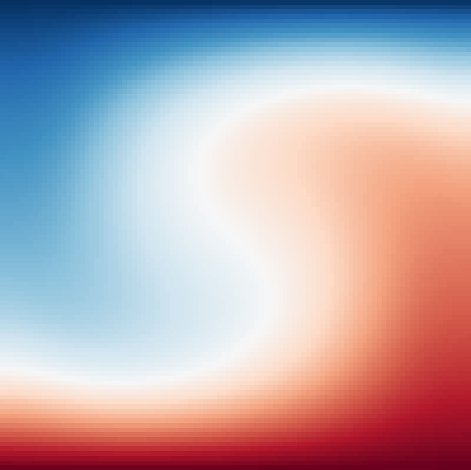
\includegraphics[width=9.99cm]{fig/rayleigh/T_no_control.png}};

	%%% probes
	\foreach \x in {0,...,7}
		\foreach \y in {0,...,7}
			\node[probe] at (0.5*1.25+1.25*\x,0.5*1.25+1.25*\y) {} ;
			
	%%% bottom frame
	\draw[fill=white] (0,-1) rectangle (10,0);
	\draw[dash pattern=on 2pt] (0,-0.5) -- (10, -0.5);
	\foreach \x in {1,...,9}
		\draw[dash pattern=on 1pt] (\x,-1) -- (\x,0);
		
	\draw[blue, thick] (0,-0.8) -- (1, -0.8);
	\draw[blue, thick] (1,-0.6) -- (2, -0.6);
	\draw[red,   thick] (2,-0.3) -- (3, -0.3);
	\draw[blue, thick] (3, -0.6) -- (4, -0.6);
	\draw[red, thick] (4,-0.2) -- (5, -0.2);
	\draw[red, thick] (5,-0.1) -- (6, -0.1);
	\draw[red, thick] (6,-0.3) -- (7, -0.3);
	\draw[blue, thick] (7,-0.7) -- (8, -0.7);
	\draw[blue, thick] (8,-0.9) -- (9, -0.9);
	\draw[blue, thick] (9,-0.6) -- (10, -0.6);

\end{tikzpicture}
%%%%%%%%%%%%
\caption{\textbf{Observation probes and actions imposition for the \codeinline{rayleigh-v0} environment}. The observations are collected at the probes regularly positioned in the domain, while the actions are imposed as piecewise-constant temperature boundary conditions on the bottom plate, with an average value equal to $\theta_H$.}
\label{fig:rayleigh_sketch_env}
\end{figure}
%%%%%%%%%%%%
%%%%%%%%%%%%